\documentclass[../main.tex]{subfiles}
\graphicspath{{\subfix{../images/}}}


\begin{document}
\chapter{Description of the physical system}

\tab In the current chapter, the basic techniques which make quantum computation using cold, confined ions feasible, are being analyzed. We are going to list the atoms that are appropriate for the implementation of the trapped-ion model, as well as the properties that allow us to create and measure efficiently two-level quantum systems. In addition, we discuss cooling and trapping techniques, which are critical for initialization and controlling of the atoms. In order to approach these topics in a methodical and precise manner, it is relevant to recall DiVincenzo's criteria\cite{DiVincenzo-criteria} for a working quantum computer, which are listed in the following section.

\section{DiVincenzo's five criteria for a working quantum computer}

%% From quantum computing devices
\begin{enumerate}
    \item The system must have well-defined qubits, and be scalable
    \item The system must have long coherence times, to permit the quantum mechanical phase of the system wavefunction to be preserved through the many steps of computation so that the error-rate must be sufficiently low.
    \item Universal quantum gates must be possible to perform all elementary logical operations.
    \item There must be an efficient means to measure the states of the qubits. At the end of a calculation, the state of each qubit state must be measured.,
    \item The system must be initialized reliably. Initialization sets the quantum system to a reproducible reference state. 
\end{enumerate}

%% Infodumping
\section{Preparation of the physical system}

\subsection{Choosing the atoms}
\tab According to the 1st Divincenzo's criterion, the system must have well-defined qubits, and also it must be scalable. In order for this statement to be satisfied, we have to find atoms or groups of atoms that are appropriate for the implementation of a system that has at least two possible states: a ground state ($\ket{g} \equiv \ket{0}$) and an excited state ($\ket{e} \equiv \ket{1}$). 
\par
In principle, any atom that has at least one electron can satisfy this condition. In practice though, since light-matter interaction 
is central to atomic physics systems, and interaction between light and the valence electron of the atom is of specific interest, it is important that we choose groups of atoms that have a single electron in the valence band, in order to create a quantum two-level system. Therefore, we are led to choose atoms from the group IA of the periodic table (i.e. alkali metals) or atoms that after ionization have one electron in the valence band. Those atoms belong in the groups IIA (alkaline earth metals), and IIIB (Transition metals).
\par 
It is significant to distinguish the advantages and liabilities of each group as per the different methods they require for control, cooling, the energy that is required for the excitation of the valence electron, and other potentially useful properties.

\subsubsection{Alkali metals}
In order to confine Alkali metals (neutral atoms) magnetic and optical forces need to be exerted upon them.\cite{PhysRevLett.91.010407} The typical depth of these traps is $\sim 1 K$, meaning that in order to trap neutral atoms effectively, we need to create Bose-Einstein condensates of those atoms, in addition to generating strong magnetic fields. The cooling techniques used in neutral atoms are, Doppler cooling and evaporative cooling, the former of which we are going to describe in detail later.

\subsubsection{Alkaline earth metals}
Alkaline earth metals (charged ions) can be trapped by generating coulomb forces. The generated electric field (typically 100 V/mm) creates a trap with typical depth $\sim 10^4 K$, meaning that charged ions can be trapped effectively at room temperatures.

\subsubsection{Transition Metals, Ytterbium-171}
The cooling and trapping methods for the case of transition metals are analogous to that of the alkaline earth metals. The major drawback of transition metals is that the energy required for the excitation of the valence electron is in the order of $\sim 10$ eV, meaning that in order to produce the excitations a laser that produces photons of appropriate wavelength ($\sim 100$ nm) coherently and with a low margin of error, is required. In order to create an efficient quantum computing device, it is relevant to minimize the required energy used for the valence electron excitations, and this property of transition metals is a limiting factor.
\par Next, we will be considering the case for Ytterbium ions (and specifically Ytterbium-171), since it has properties that are appealing for the ion trap configuration. 
A significant advantage Ytterbium atoms have over other transition metals is that the excitation energy of the valence electron is relatively lower, and laser light in the visible spectrum can be used for the excitations. This property allows for efficient initialization of all qubits by utilizing  currently available technologies for light transmission (i.e. optical fibers). Another useful property is that it has a hyperfine structure, which is defined by small shifts in otherwise degenerate energy levels and the resulting splitting in those energy levels of ions, due to electromagnetic multipole interaction between the nucleus and electron clouds. These properties make Ytterbium 171 ions an excellent qubit candidate.\cite{PhysRevA.76.052314,10.1116/5.0065951}


\subfile{cooling}

\subsection{Trapping Ions}
In the ion-trap model, independent manipulation of each individual qubit is accomplished by directing different laser beams to each of the ions. The coupling of the motion of the ions is provided by the Coulomb repulsion, which is much stronger than any other interaction for typical separations between the ions, and allows for creating traps that have a depth $\sim 10^4 $ Kelvin. The charge has major differences when confining and manipulating particles. Comparing them, the force exerted on neutral ions are magnetic and optical forces, typically the traps that are created have a depth $\sim 1$ Kelvin.

\subsubsection{Penning Ion Trap}
The Penning ion trap uses a quadrupole potential in order to confine a charged particle axially, with a 3-dimensional minimum potential
\begin{equation}
    \phi(x,y,z) = Ax^2 + By^2 + Cz^2
\end{equation}

\noindent where A, B, C are all positive. However, the Laplace equation $\nabla^2 \phi = 0$ requires that $A + B + C = 0$, rendering a 3-dimensional trapping with a static field not possible. 

\begin{figure}[ht!]
    \centering
    \begin{subfigure}{0.45\textwidth}
        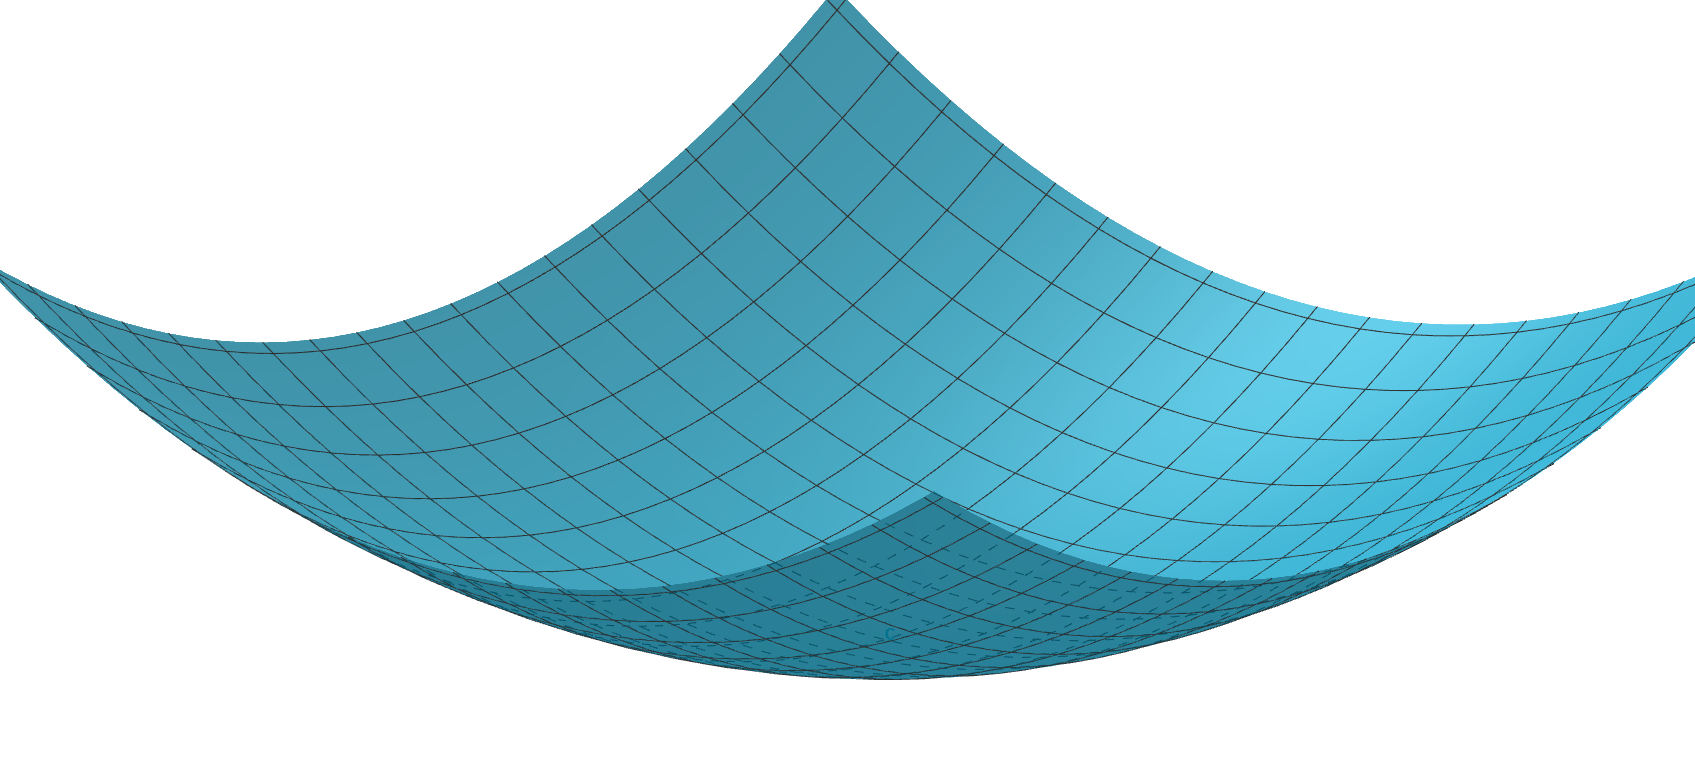
\includegraphics[scale = 0.15]{images/desired potential well.png}
        \caption{}
        \label{fig: desired potential well}
    \end{subfigure}
    \begin{subfigure}{0.45\textwidth}
        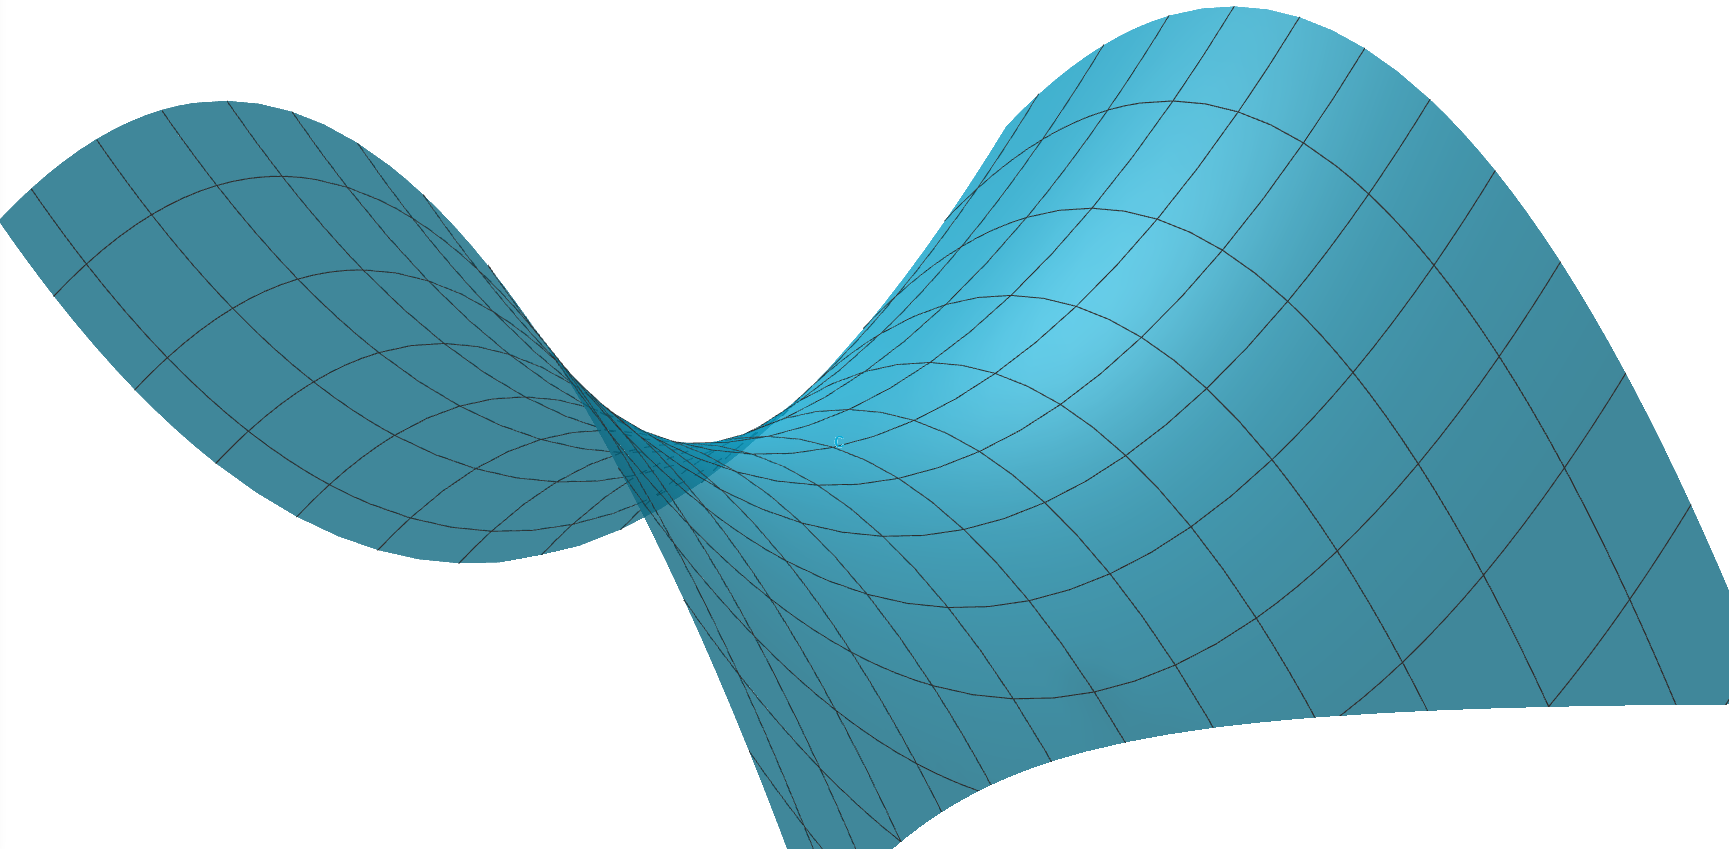
\includegraphics[scale = 0.15]{images/actual potential well.png}
        \caption{}
        \label{fig: actual potential well}
    \end{subfigure}
    \caption{The confining potential well (a) and the potential well of a static electric field (b)} 
\end{figure}

In order to solve this problem, a uniform magnetic field is introduced, the Lorentz forces of which could be used for confinement of the ion in the radial plane. The Lorentz forces transform the radial motion of the ion into a cyclotron motion. The motion of the charges in the joint potential is basically harmonic, having well-defined frequencies, satisfying the Cirac-Zoller (and DiVincenzo) conditions for a quantum computer. However, the uniform magnetic field for effective ion confinement, and must not charge in space-time over the region in space where the ions are confined to preserve coherence. The stability of a magnetic field, which affects the energies of the magnetic sublevels of an ion electronic state by the Zeeman effect, may compromise wavefunction coherence unless carefully controlled. These conditions can be difficult to meet.

\begin{figure}[!ht]
    \centering
    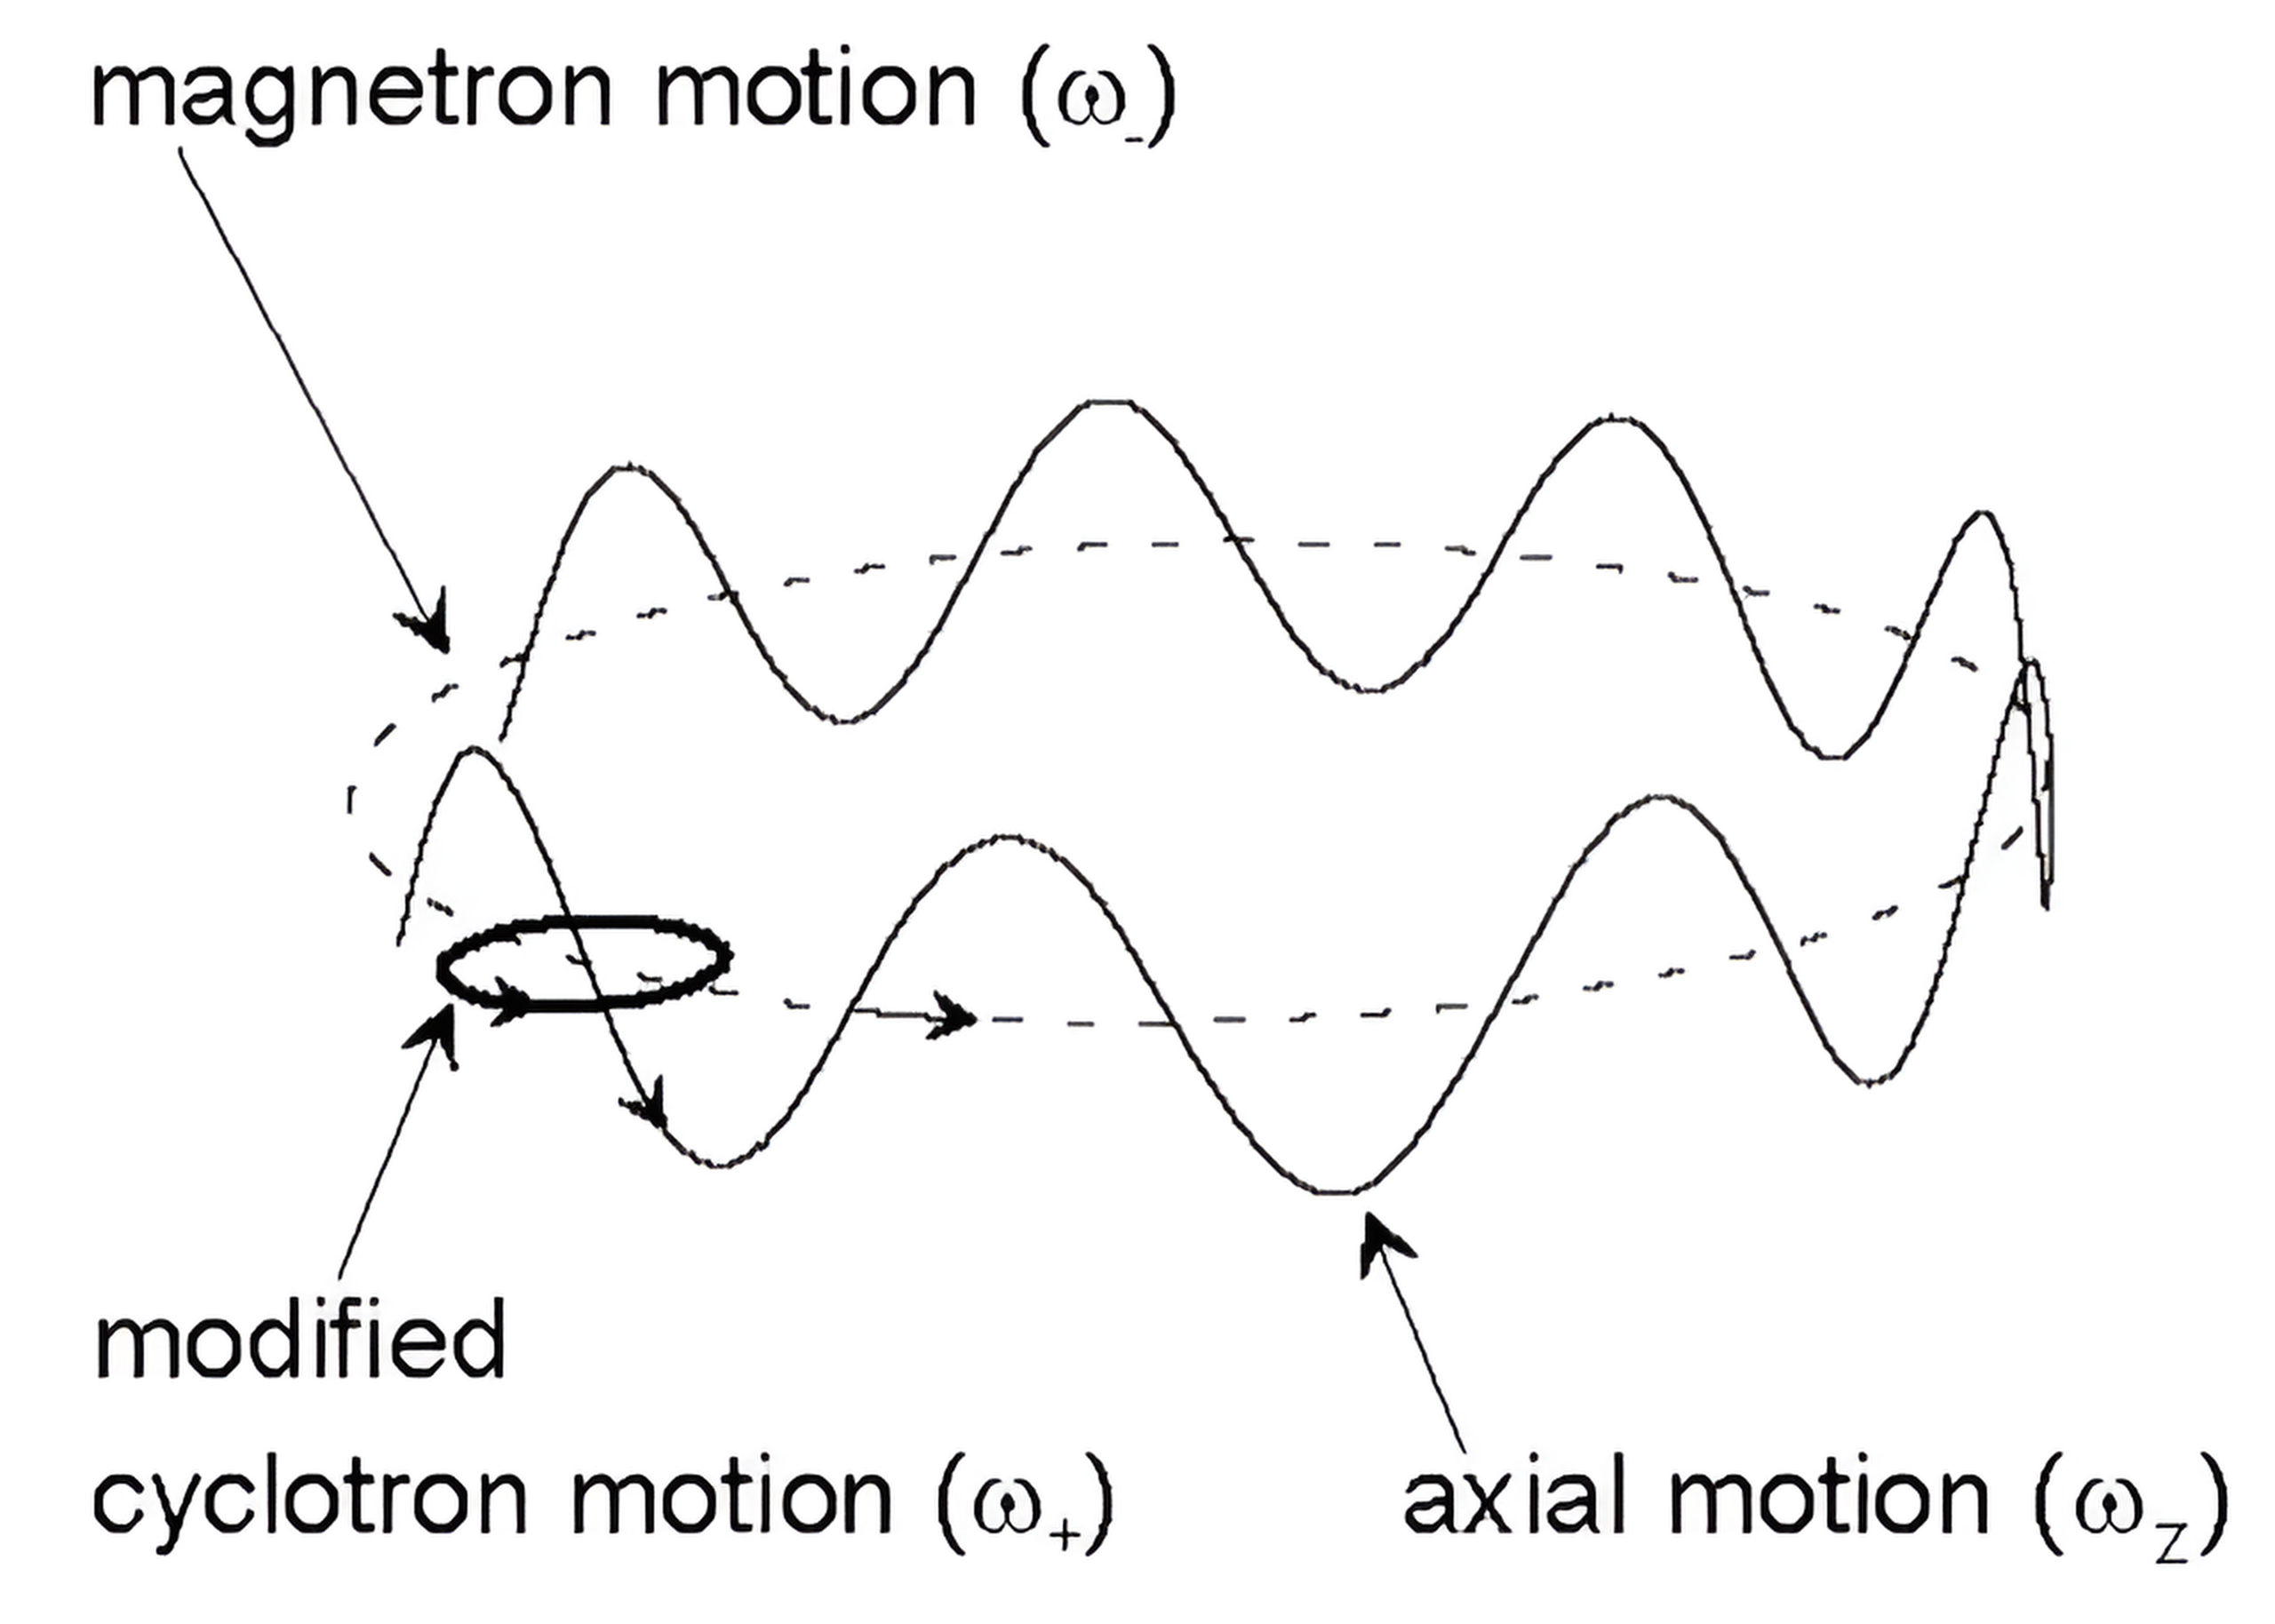
\includegraphics[scale = 0.12]{images/penning trap.png}
    \caption{Characteristic ion motions in a Penning Trap. Source: \href{https://www.med.physik.uni-muenchen.de/research/nuclear-science/nuclear-masses/mlltrap/layout/traps/index.html}{LMU}}
\end{figure}

\subsubsection{Radio Frequency Trap}

The radio frequency ion trap (or Paul trap) is chosen for quantum computation for several reasons. It provides a stable 3-dimensional minimum in space of the effective electric potential using only radio frequency and DC electric fields. A magnetic field may additionally be imposed, but is not required for confinement, and can be kept small. Since the electric fields vanish at the potential minimum, the effects on the energies of the ion electronic levels by the Stark effect\cite{STARK1913} is very small, when the ions are cold. The motion of very cold ions in the trap is harmonic, i.e., the restoring force toward the equilibrium is linear in space.

\begin{figure}[!ht]
    \centering
    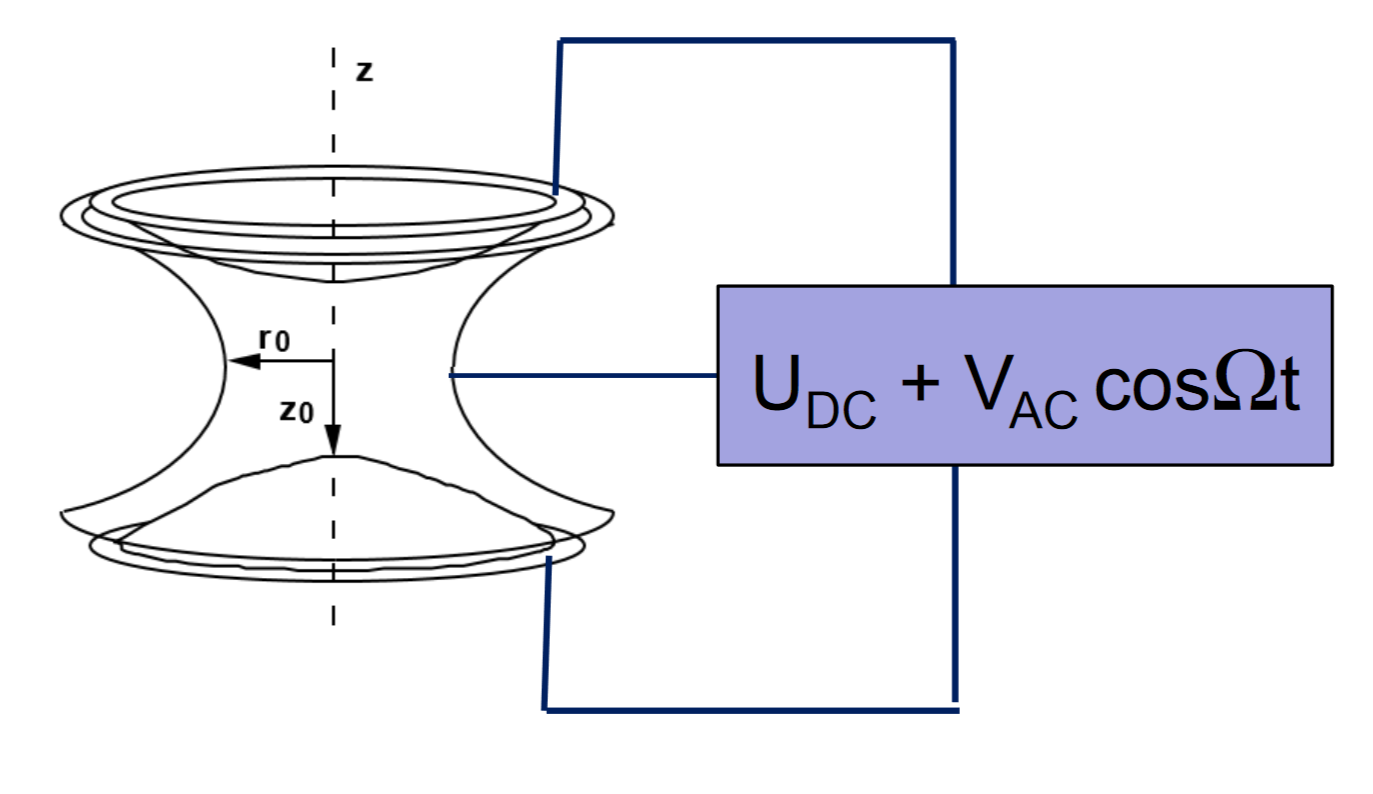
\includegraphics[scale = 0.2]{images/paulTrapApparatus.png}
    \caption{The Paul trap consists of a ring and 2 endcaps of hyperboloid shape. An oscillating voltage between the electrodes is applied in order to effectively produce a rotating potential well that confines the ion at the minimax point of the potential well. The resulting potential is $\phi(x,y,z,t) = (U_{DC} + V_{AC}\cos{\rf t})(x^2 + y^2 + 2z^2)/(2r_0^2)$. Source: \href{https://indico.cern.ch/event/315947/sessions/61194/attachments/606588/834751/Paul_traps_until_page_79.pdf}{Martina Knoop, CNRS/Université d’Aix-Marseille}}
    \label{fig: paul trap device}
\end{figure}


\par In order to accomplish the confinement of multiple qubits we could use a linear Paul trap design, which is an analogue of \cref{fig: paul trap device}. With the ions confined in a cylindrical space within four linear conducting electrodes oriented along the $z$-axis, the z component of the potential is suppressed. As a result, the time-varying electric quadrupole potential within the volume defined by the rods, produces a spatially non-uniform time varying electric field which is described by the following equation:
\begin{equation}
    \phi(x,y,t) = (U - V\cos{\rf t})\frac{(x^2-y^2)}{2r_0^2}
\end{equation}

\noindent A time-varying potential $\frac{V}{2}\cos{\Omega_{\text{rf}}t}$ is applied to two opposite electrodes, and $-\frac{V}{2}\cos{\Omega_{\text{rf}}t}$ to the other opposite pair, or alternatively $V\cos{\Omega_{\text{rf}}t}$ is applied to one electrode pair and the other pair is grounded, an electrically simpler equivalent arrangement.

\begin{figure}[!ht]
    \centering
    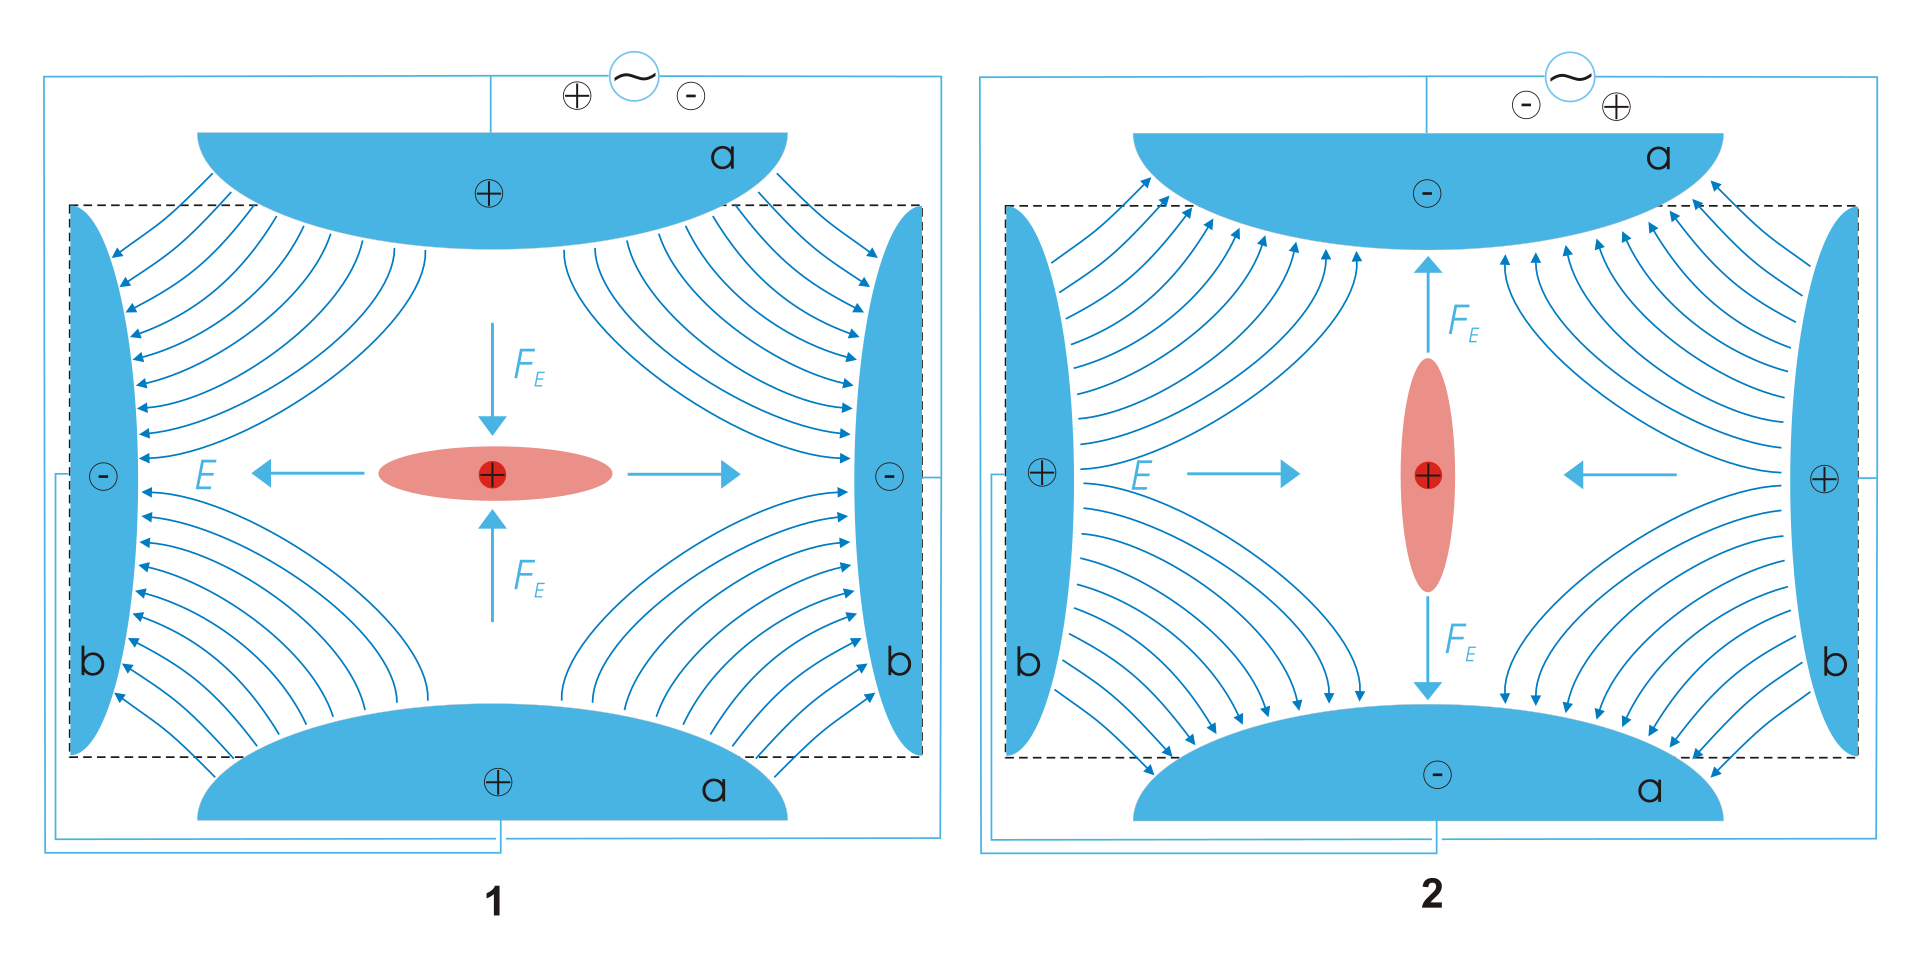
\includegraphics[scale = 0.18]{images/1920px-Paul-Trap.svg.png}
    \caption{Scheme of a quadrupole ion trap of classical setup with a particle of positive charge (dark red), surrounded by a cloud of similarly charged particles (light red). The electric field E (blue) is generated by a quadrupole of endcaps (a, positive) and a ring electrode (b). Picture 1 and 2 show two states during an AC cycle. Source: \href{https://en.wikipedia.org/wiki/Quadrupole_ion_trap}{Quadrupole Ion Trap}}
\end{figure}

\par
The motion of the ions in the linear Paul trap along the $z$ axis can be confined, by using a positive DC potential that increases the positive ion moves in either direction along the $z$ axis away from the linear trap center. Since the Laplace equation 
\begin{equation}
    \nabla^2 V_{DC}(x,y,z) = 0
\end{equation}

\noindent must also be satisfied, there is additionally a modification in the transverse frequency $\omega$ due to the DC potential. The result is overal harmonic confinement of the ions in all three dimensions but with different frequencies in different dimensions. 

\begin{figure}[!ht]
    \centering
    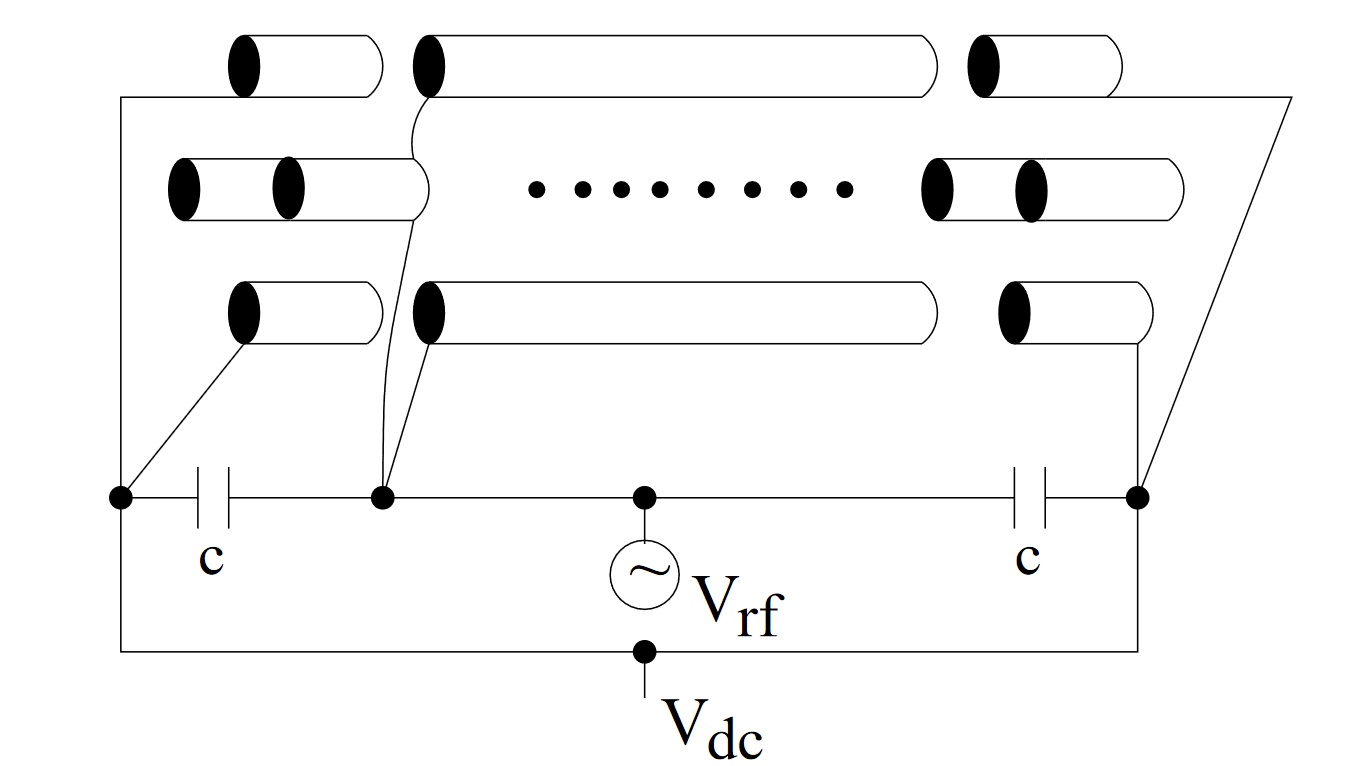
\includegraphics[scale = 0.3]{images/linearPaulTrap.png}
    \caption{\cite{Englert2006QuantumCD} Illustration of axial confinement in a linear RF trap. The gap in the rod structure permits a DC voltage on the ends of the rods, while capacitors C permit the RF voltage on all parts of the structure. A similar bias arrangement holds for the two rods not shown. A string of cold confined ions is shown as black dots.}
\end{figure}

\noindent Overall, the ions in the linear array are separated axially by a balance between the Coulomb repulsion of the charges, and the force exerted by the confining axial electric field. The equilibrium ion spacing of the ions along the z axis tends to decrease near the trap center. Nevertheless, ion separations in the array are measured in micrometers, while zero point oscillation amplitudes of cold ions are measured in nanometers, and ion internal state wave function distributions having significant probability in space are still smaller. This means that each ion is physically isolated from the others in the array unless a deliberate coupling is externally initiated.



\end{document}